% ===== §4 The Formal Criterion of Generative Effacement =====
\section{The Formal Criterion: Phase Capture and the Loss of One's Own Frequency}
\label{p18:sec:criterion}

\noindent
The harm named in \xref{p18:sec:definition} is invisible to every metric the prior literature supplies. A distributive metric records that one party holds less; here the difficulty is that aggregate value is \emph{rising}. A recognitive metric records that one party is misrecognised; here she may be fully and warmly recognised. An epistemic metric records that one party cannot be heard; here she is heard and thanked. What is required is a criterion that registers a harm consistent with rising value, sincere recognition, and full audibility---a criterion not of holdings, status, or intelligibility, but of whether the other still generates \emph{as herself}. This section constructs such a criterion and shows that it is not a gradient shading imperceptibly out of health but a \emph{phase boundary} that can be located exactly.

\subsection{Two independent dimensions}
\label{p18:sub:crit-two}

A single distinction organises the chapter. The \emph{topology of coupling}---how two generating subjects coordinate---and the \emph{survival of generation}---whether each still generates at its own rhythm---are independent axes. The series' coupling typology classifies the first; the criterion of this paper concerns the second. The standard error, which the section exists to forestall, is to read a strong and harmonious coupling as evidence of health. Coupling can be strong, harmonious, and mutually willed, and the weaker party can nonetheless have ceased to generate as herself.

The coupling typology gives four regimes, by whether the two subjects pursue the same or different goals and whether their coupling is high or low-with-high-dynamical-diversity: (1)~same goal, high coupling---a joint sprint, force possibly unequal; (2)~same goal, low coupling and high diversity---complementary work on one complex problem; (3)~different goals, high coupling---a parallel sprint; (4)~different goals, low coupling and high diversity---complementary parallel work on many problems. These four are regimes of \emph{health}: in each, both poles retain a non-zero generative rhythm. \emph{Effacement is not a fifth regime.} It is the common degenerate limit into which any of the four can collapse when one pole loses its own rhythm---and, as the model shows, the collapse is governed not by which regime one is in but by two quantities that cut across all four.

\subsection{The model}
\label{p18:sub:crit-model}

Represent each subject as a phase oscillator---the minimal model of a system with its own intrinsic rhythm of generation. Let $\theta_w$ and $\theta_s$ be the phases of the weaker and stronger pole, with intrinsic frequencies $\omega_w$ and $\omega_s$, the rate at which each, left alone, generates. The stronger pole is the one with the higher intrinsic frequency, $\omega_s>\omega_w$: it generates faster.

Two parameters describe their relation. The \emph{coupling strength} $K$ measures how strongly each pole's state is pulled toward concordance with the other. The \emph{force asymmetry} $\Delta\in[0,1]$ measures the directedness of that pull: the traction exerted \emph{on} the weaker pole is $K(1+\Delta)$, that on the stronger $K(1-\Delta)$. At $\Delta=0$ the coupling is symmetric; as $\Delta\to1$ the weaker pole is fully subject to the stronger while the stronger evolves freely. The dynamics are
\begin{align}
  \dot\theta_w &= \omega_w + K(1+\Delta)\,\sin(\theta_s-\theta_w),\\
  \dot\theta_s &= \omega_s + K(1-\Delta)\,\sin(\theta_w-\theta_s).
\end{align}
The phase difference $\varphi=\theta_w-\theta_s$ obeys an Adler equation,
\begin{equation}
  \dot\varphi = (\omega_w-\omega_s) - 2K\sin\varphi,
  \label{p18:eq:adler}
\end{equation}
whose behaviour gives the criterion directly.\footnote{The reduction to a single Adler equation \eqref{p18:eq:adler} follows because the two traction terms, $K(1+\Delta)$ and $K(1-\Delta)$, enter $\dot\varphi$ additively and sum to $2K$ independently of $\Delta$. Thus $\Delta$ drops out of the \emph{locking condition} and survives only in the location of the locked frequency---the formal root of the two-structure result of \xref{p18:sub:crit-result}. On the Kuramoto reduction generally see \textcite{kuramoto1984}.}

\subsection{The order parameter and the criterion}
\label{p18:sub:crit-order}

The criterion must measure not how \emph{much} the weaker pole generates but whether what it generates is \emph{its own}. The order parameter is therefore the degree to which the weaker pole's realised rate departs from its own intrinsic frequency and is drawn toward the stronger's:
\begin{equation}
  E \;=\; \frac{\dot\theta_w^{\,\text{realised}} - \omega_w}{\omega_s - \omega_w},
  \qquad E\in[0,1].
  \label{p18:eq:order}
\end{equation}
$E=0$ means the weaker pole advances at its own frequency---it generates as itself. $E=1$ means its realised rhythm has been pulled entirely onto the stronger's frequency---it is in motion, but the motion is the echo of another's rhythm, not its own generation.

\begin{claim}[Effacement as the loss of one's own frequency]
Generative effacement is not the cessation of a subject's activity but the replacement of its own generative rhythm by another's. The effaced pole still moves; an outside observer sees a harmonious, active, synchronised pair. What the observer cannot see, and the order parameter $E$ can, is that one of the two rhythms has gone silent and been overwritten by a copy of the other. This is why the harm is consistent with rising value and reported harmony: the motion, and the value it produces, are real---only they are no longer \emph{hers}.
\end{claim}

\subsection{The result: two distinct structures}
\label{p18:sub:crit-result}

Integrating the model across the $(K,\Delta)$ plane (Figure~\ref{p18:fig:phase}) yields a result sharper than a gradient of risk, and the sharpness is the section's main technical claim. \emph{Two distinct structures govern the harm, and they must not be conflated.}

\textbf{First, whether effacement occurs at all is governed by $K$ alone.} Equation~\eqref{p18:eq:adler} locks---the weaker pole loses its own frequency---if and only if
\begin{equation}
  K \;\ge\; K_{\text{lock}} \;=\; \frac{|\omega_s-\omega_w|}{2}.
  \label{p18:eq:klock}
\end{equation}
This is a genuine phase transition with an exact threshold, and it is \emph{independent of $\Delta$}. Below $K_{\text{lock}}$ the weaker pole keeps its own rhythm however asymmetric the coupling; above it, the weaker pole is captured. The boundary is the vertical dashed line in Figure~\ref{p18:fig:phase}. To its left lies the \emph{autonomous regime}; to its right, the \emph{collapse region}.

\textbf{Second, once capture has occurred, how deeply the weaker pole is effaced is governed by $\Delta$.} In the locked state the common frequency is the traction-weighted mean of the two intrinsic frequencies, and the normalised effacement is
\begin{equation}
  E \;=\; \frac{1+\Delta}{2}.
  \label{p18:eq:edepth}
\end{equation}
This is the vertical gradient within the collapse region: at fixed super-threshold $K$, the harm deepens monotonically with force asymmetry, from $E=\tfrac12$ at $\Delta=0$ to $E\to1$ as $\Delta\to1$.

\begin{claim}[Equal power does not protect the weaker pole]
Set $\Delta=0$---perfectly symmetric, equal-force coupling, the very picture of a balanced union---and read along the bottom edge of Figure~\ref{p18:fig:phase}. Effacement is still $E=\tfrac12$ for every $K$ above threshold. As long as the two subjects have different intrinsic rhythms and the coupling is strong enough to lock them, the slower is drawn off its own frequency by half the gap, \emph{regardless of any equality of power}. Force asymmetry $\Delta$ decides only \emph{which} pole is sacrificed more and \emph{how far}; it is coupling strength $K$, not inequality of force, that decides \emph{whether} a pole is sacrificed at all. The harm is, in the first instance, a property of strong coupling between unlike rhythms---not of unequal power.
\end{claim}

\begin{figure}[t]
\centering
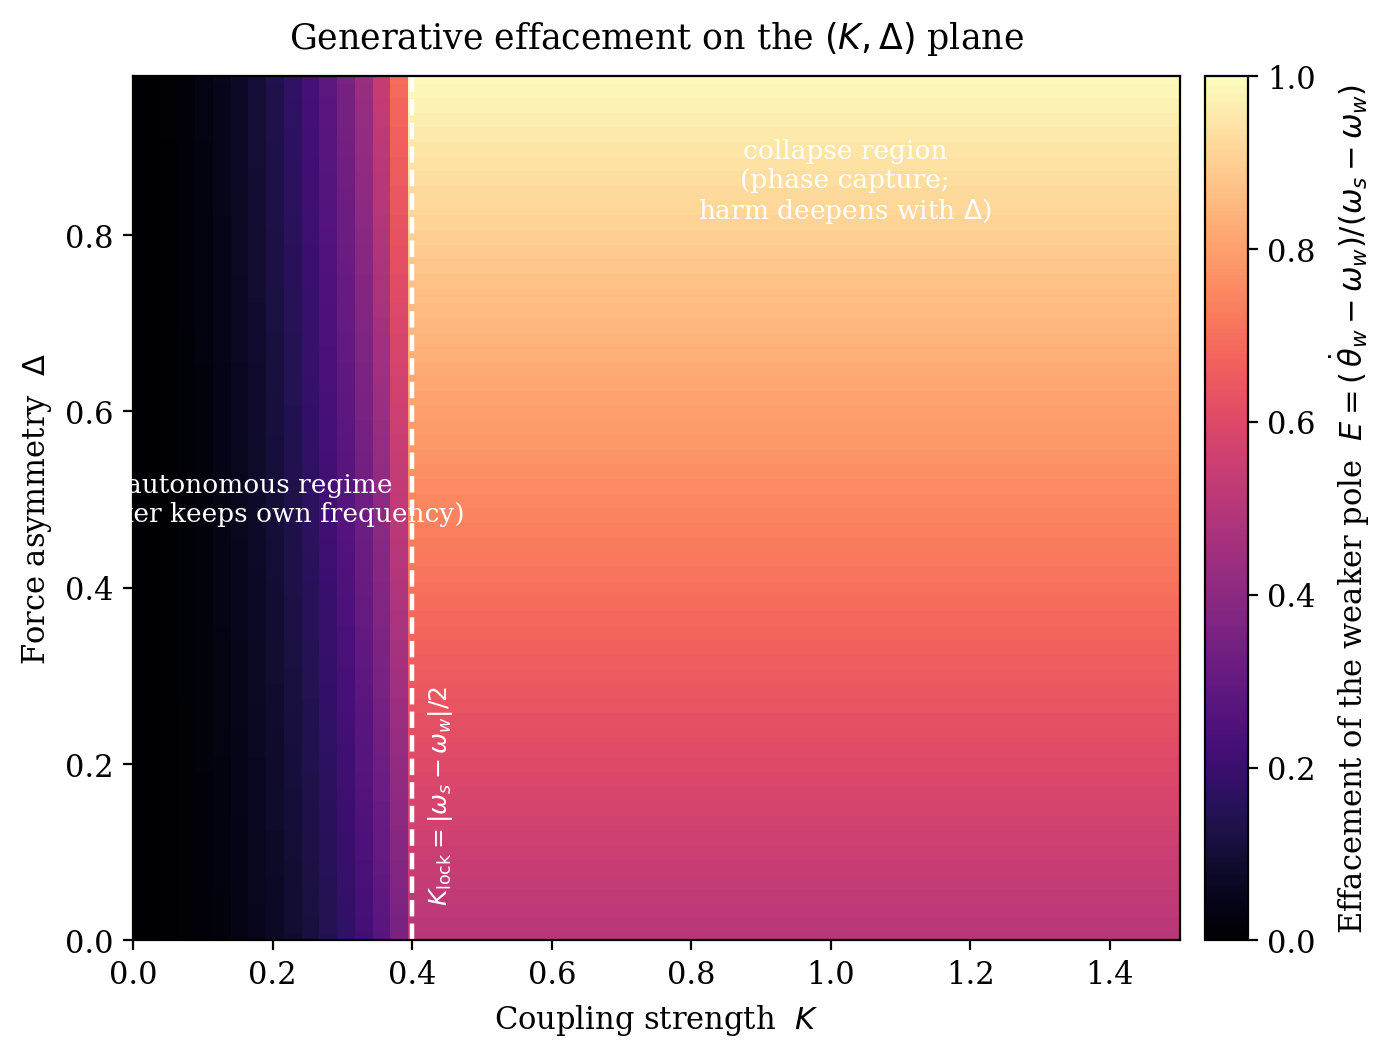
\includegraphics[width=0.96\linewidth]{figures/phase_diagram.png}
\caption{Effacement $E$ of the weaker pole on the $(K,\Delta)$ plane. Vertical dashed line: the locking threshold $K_{\text{lock}}=|\omega_s-\omega_w|/2$ of \eqref{p18:eq:klock}, independent of $\Delta$. \emph{Left:} the autonomous regime---the weaker pole keeps its own frequency ($E=0$). \emph{Right:} the collapse region---the weaker pole is phase-captured and the harm deepens with $\Delta$ by \eqref{p18:eq:edepth}, reaching $E=1$ as $\Delta\to1$. Note the bottom edge: at $\Delta=0$ (equal force) effacement is still $E=\tfrac12$ throughout the collapse region. Equal power does not prevent capture.}
\label{p18:fig:phase}
\end{figure}

\subsection{Three readings of one degeneration}
\label{p18:sub:crit-three}

The same transition can be read in the three idioms the series has already built, which is the warrant for treating it as one phenomenon rather than an analogy.

\emph{Predictive coding} (\cite{paperxiii}; \cite{paperxi}). The stronger pole, generating and pre-arranging faster, pre-symbolises the shared future, driving the weaker pole's prediction error toward zero. Active inference---the generation of new value---feeds on unresolved uncertainty; with the future pre-determined, the fuel is gone. Phase capture is, in this idiom, the foreclosure of the weaker pole's predictive horizon. This extends \pinkref{Paper~XVII}'s claim \parencite{paperxvii} that desire withholds itself from total symbolisation in order to remain alive: here one subject's over-symbolisation extinguishes another's.

\emph{Holonomy} (\cite{paperix}; \cite{paperxi}). Above threshold the system's aggregate holonomy is positive---value genuinely accumulates---while the captured pole's own phase advance, measured against its intrinsic frequency, has collapsed. This is the \emph{single-subject spiral}: a system ascending on one pole's rhythm alone. It is the limiting case of \pinkref{Paper~XI}'s justice-as-skewness, the skew carried to the point where one distribution has lost its variance entirely.

\emph{Coupling} (the present contribution): phase capture above $K_{\text{lock}}$, with depth set by $\Delta$, as derived above.

\subsection{The inversion}
\label{p18:sub:crit-inversion}

The result overturns the common identification of intimacy with strong coupling and of strong coupling with good. Strong coupling presents itself as union---\emph{we move as one}---and it is precisely strong coupling that, between unlike rhythms, captures the weaker pole and silences its frequency. Low coupling with high dynamical diversity presents itself as distance, and it is precisely what lets two unlike rhythms each survive.

\begin{claim}[The inversion of the intimacy criterion]
The good of intimacy is not the strength of the coupling but whether the coupling leaves each pole turning at its own frequency. This is the same law \pinkref{Paper~XVII} reached from another direction in identifying perfect concordance with equilibrium and equilibrium with death: a relation at perfect, frictionless agreement is one in which one of the two rhythms has stopped. High coupling is not the measure of love but, between unlike rhythms, its most common solvent.
\end{claim}

\subsection{The criterion stated, and its handoff to justice}
\label{p18:sub:crit-handoff}

The formal criterion of generative effacement is therefore: \emb{a co-generative relation effaces its weaker pole when its coupling exceeds the locking threshold $K_{\text{lock}}$, drawing that pole off its own intrinsic frequency; the depth of effacement is $(1+\Delta)/2$.} The criterion is satisfiable, and is in fact at its most dangerous, when aggregate value rises and both parties report harmony---exactly the case \xref{p18:sub:crit-two} required it to catch.

This hands \xref{p18:sec:reticence} a justice with a precise operational meaning. If the harm is crossing $K_{\text{lock}}$, the remedy is to return below it: to lower the coupling until the weaker pole recovers its own frequency. Crucially, the threshold \eqref{p18:eq:klock} depends on $K$, not on the stronger pole's frequency $\omega_s$. The stronger pole need not slow its own generation---lowering $\omega_s$ is neither necessary nor, by itself, sufficient. What restores the weaker pole is lowering $K$: releasing the traction, not reducing the speed. That distinction, derived here, is the whole content of the claim in \xref{p18:sec:reticence} that the justice of reticence is \emph{decoupling, not deceleration}.
